\newcommand{\mypathmsip}{../thesis/msip}
\newcommand{\mypathmsipdata}{../thesis/msip/data}
\chapter{Modeling Cascading Power Failures}\label{msip-model}
An ideal model is complex enough to capture the important features and effects of the process, while remaining simple enough to work with and remain believable.  Arbitrarily complex models can be made to produce the output matching nearly any process, but often there is no reason to believe that the individual mechanisms being modeled are important or represent a real part of the process.  In this chapter, we review a simple simulation model for estimating the load shed from a cascading power failure.  We analytically capture the relevant features of the simulation model into a mixed-integer stochastic program (MISP) with decision-dependent uncertainty.  Our MSIP can be embedded in a variety of optimization problems designed to mitigate the effects of cascading power failures.

\section{Literature Review}
Historically, cascading power failures have been a hard problem to understand, and since they are rare, the process was not studied much.  However, after the Northeast Blackout of 2003, more focus has been devoted to this problem.  

The simplest models of the cascading process are strictly topological models with some mechanism to fail components such as a failed node leads to its neighbors to fail with a given probability.  While these models can capture interesting effects due to degree distribution and clustering, they lack important information about the electrical parameters of the topology as well as loading patterns.   

After discussing historical topological models, Hines, Cotilla, {\it et. al.} \cite{hines_2010}, \cite{cotilla_2012} provide a rebuttal to strictly topological models.  Here, topological measures are looked at in addition to the electrical information behind the topology of the grid. 
%Then, pseudo-topological measures such as electrical distance and centrality will be developed and their importance discussed.

Finally, the Oak Ridge National Laboratory, Power System Engineering Research Center of Wisconsin University, and Alaska University (OPA) type models are developed.  These models use the electrical parameters as well as demand and generation information to solve the power flow problem.  The results of this are loading patterns on the topology of the power grid.  Using these loading patterns as well as a deterministic or probabilitic failure mechanism, another level of complexity can be added to the cascading failure model.  The following quote from Hines et. al. \cite{hines_2011} supports the use of this type of model.

\begin{quote}
While a perfect model of cascading failure would accurately represent the continuous dynamics of rotating machines, the discrete dynamics associated with relays that disconnect stressed components from the network, the non-linear algebraic equations that govern flows in the network, and the social dynamics of operators working to mitigate the effects of system stress, all power system models simplify these dynamics to some extent. Unlike simple topological metrics, our model does capture the effects of Ohm's and Kirchhoff's laws, by using linear approximations of the non-linear power flow equations \cite{bergen_1986}. Similar models have been used to study cascading failure in a number of recent papers \cite{carreras_2004}, \cite{dobson_2007}, \cite{mei_2009}.
\end{quote}

In addition to the fast time scale cascading model, the OPA work included a slow time scale model, which responded to these cascading failures by engineering improvements.  It is the dynamic interactions of these two forces that leads to an equilibrium in which blackouts of all sizes occur and the size follows a power law distribution.

In order to use OPA models, power flows need to be calculated and to reduce the computational complexity of the model, a Decoupled (DC) power flow model is used by making a few simplifying assumptions.  Using the power flow model, an economic dispatch model can be made to dispatch the generators at least cost, while remaining within its operating constraints.  This dispatch model is used to connect the reliability issues of the power grid with economic ones.
%First, the balanced three phase AC power flow equations will be discussed along with its strengths and weaknesses. 

\subsection{Topologic Model}

This section first discusses historical topological models and then describe common topological measures.  These measures are used to compare to other network structures.  Using these measures, it is shown that power grids differ from many other common network structures and thus need to be analyzed on their own.  

\subsubsection{Historical Topological Models}
In 2004, Albert et. al. \cite{albert_2004} worked on large blackouts in response to August 2003 and developed a deterministic model of failures based on topological measures.  They used 4 methods of removing nodes from the grid one at a time, randomly, highest degree, highest load, and cascading.  The main simplifying assumption is that if a generator is connected to a load, its power is available.  In addition, power is routed along the shortest path from generation to load.  Then, in order to monitor the effects of the failure patterns, connectivity loss is recorded, which represent the average decrease in number of generators connected to a substation.  They conclude by noting possible solutions of increasing redundancy and capacity of the system or decreasing reliance on transmission by using more generation at the distribution substation level.

Kinney and others developed another method for estimating power flows on a given topology \cite{kinney_2005}.  They introduce the concept of efficiency for power lines and use the harmonic composition of the efficiency of lines to calculate an efficiency measure for any given path.  Now, the electricity is distributed to a load from a generator along the most efficient path.  Then, they modeled an efficiency degradation based on loading through time as well as tolerance measures to fail lines probabilistically.

A handful of these topological models with flow estimates were done in between 2003 and 2010.  Some were predicated on behaving like other networks such as scale-free networks \cite{zhao_2004}, \cite{wang_2009} or small-world networks \cite{ding_2006}.  Others used matching models with a profit function to protect against cascading failures \cite{sun_2008} or novel recourse strategies such as deliberate weak lines for network islanding \cite{duenas-osorio_2009}. 

\subsubsection{Topological Measures}

The topology of a power grid can be described as an unweighted, undirected graph $\cG$ with vertices $\cV$ and edges $\cE \subset (\cV \times \cV)$ that connect the vertices.  A particular grid is denoted by a subscript, such as $\cG_{EI} = \left\{ \cV_{EI}, \cE_{EI} \right\}$, which would be the graph that represents the Eastern Interconnect.  The vertices $\cV$ on the graph can represent demand nodes, generator nodes, and buses in the transmission network.  The edges $\cE$ represent elements such as transmission lines and transformers.  For convenience, we define $n_v = \magV$ and $n_e = \magE$.

A useful tool for describing topological measures on graphs is the adjacency matrix, $A$.  The elements $a_{ij}$ of $A$ represent whether nodes $i$ and $j$ are connected, such that if $(i,j) \in \cE$ then $a_{ij} = 1$, else $a_{ij}=0$.  The degree $k_i$ of a node measures how connected it is to the rest of the network, with
\begin{equation}
k_i = \sum_{j=1}^{n_v} a_{ij}
\end{equation}
A common measure to compare different graphs is the average degree $\hat{k} = 2 n_e/n_v$.  Cotilla et. al. \cite{cotilla_2012}, using data for EI from NERC in 2012 and data for WI and TI from FERC in 2005, found the average degree of the networks, which is given in \Cref{tab:topo_info}.  This tells us that our power grids are sparsely connected, with around 2.5 transmission elements connecting each vertex, noting that parallel lines are counted as one.  The following statistical analysis of topological measures was done by Cotilla et. al. \cite{cotilla_2012} in order to show that power grids are neither small-world networks nor scale free networks.

\begin{table}
\centering
\begin{tabular}{| c | c c c c c c c|}
\hline
Grid & Vertices & Edges & $\hat{k}$  &  $k_{max}$ & $C$ & $L$ & $d_{max}$ \\
\hline
$\cG_{EI}$	& 41,228	&	52,075	&	2.53	&	29	&	0.068	&	31.9	&	94	\\
$\cG_{WI}$	& 11,432	&	13,734	&	2.4	&	22	&	0.073	&	26.1	&	61	\\
$\cG_{TI}$ 	& 4,513	&	5,532		&	2.45	&	18	&	0.031	&	14.9	&	37	\\
\hline
\end{tabular}
\caption{Topological measures for the three US power grids}
\label{tab:topo_info}
\end{table}


There are many statistical measures used to compare our power grid graphs to other common graph structures.  The first measure is the distribution of the degree, $k_i$, of all the nodes.  One type of network to compare to is a scale-free network which have a power-law degree distribution.  These networks have highly connected central hubs, which are inherent weak points to the network.  However, high-degree nodes are far less common in power grids than would be expected with a scale-free network.    

Two additional measures, which are distance metrics, are diameter and characteristic path length.  The distance $d_{ij}$ between $i$ and $j$ is the minimum number of links needed to traverse from vertex $i$ to vertex $j$.  The diameter is then 
\begin{equation}
d_{max} = \max_{ij} d_{ij}
\end{equation}
 and the characteristic path length is 
\begin{equation}
L = \frac{1}{n_v (n_v -1)} \sum_{\forall i,j | i \neq j} d_{ij}.
\end{equation}
In addition, the average nodal distance $\hat{d} = \sum_{j=1}^{n_v} d_{ij}$ can be used.  As the size of small-world networks increase, the characteristic path length increases roughly with $\ln n_v$, which means the distances between vertices grows slowly.  However, the power grid's path length always grows faster than $\ln n_v$ and falls between small-world networks and regular grids, which scale linearly with $n_v$.

Another useful measure is the cluster coefficient which gives insight into neighborhoods of nodes.  Let $e_i$ be the number of edges connected to vertex $i$ and its immediate neighbors $N_i$ by the following $e_i =\sum_{\forall j,k \in \left\{ N_i \cup i \right\}} a_{jk}/2$.  Then the clustering of node $i$ is
\begin{equation}
c_i = \frac{e_i}{(k_i(k_i-1))/2}
\end{equation}
and the cluster coefficient of the graph is $C = \frac{1}{n} \sum_{i=1}^{n_v} c_i$.  Power networks were found to have less clustering than small world networks but much larger than random grids, which may be due to relatively few long distance lines.

The final measure used was degree assortativity, which is the correlation of the degree of two connected nodes.  Power networks were found to have small, negative degree assortativity.  This was due to distribution feeders, which have a large number of radial lines connecting single loads to the substation.  This behavior was not found in small-world networks.

Hines et. al. \cite{hines_2010} conclude that while these topological measures are useful for understanding the structure and perhaps indicating general vulnerabilities, they can lead to erroneous conclusions.  For example, Kinney et. al. \cite{kinney_2005} and Albert et. al. \cite{albert_2004} draw different conclusions about such things as the effects of single failures using similar data.  Power flow based models are more realistic and thus more useful for vulnerability analysis.  However, analogous measures with electrical topological information can be very useful. 
%\endnote{\textbf{Pseudo-Topological Measures}

Cotilla et. al. \cite{cotilla_2012} use the fact that voltage phase angles between areas as measure of stress in power networks (47).  Using the power flow Jacobian matricies,
\begin{equation}
 \Delta P = \frac{ \partial P }{ \partial \theta} \Delta \theta + \frac{ \partial P }{ \partial | V | } \Delta | V |
\end{equation}
and assuming voltages are held constant, then $\frac{ \partial P }{ \partial \theta} $ is a Laplacian matrix.
Set the conductance matrix $G = \frac{ \partial P }{ \partial \theta}$, then with
\begin{equation}
e_{ij} = g_{ii}^{-1} + g_{jj}^{-1} - g_{ij}^{-1} - g_{ji}^{-1}
\end{equation}
$E$ satisfies properties of distance matrix under dc power flow assumption, and empiraclly held otherwise.  $E$ is weighted and fully connected with $n_v(n_v-1)$ links.

We then have a quantity that is analogous to node degree, $k_i$, called electrical distance
\begin{equation}
e_i = \sum_{j=1}^n \frac{e_{ij}}{n-1}
\end{equation}
with the inverse representing centrality
\begin{equation}
c_i = e_i^{-1}
\end{equation}

An unweighted graph can represent these distances.  Let $R$ be an adjencency matrix and by defining $r_{ij} = 1 $ if $e_{ij} < t$ and adjusting $t$ so that there are  $n_e$ links.  $R$ has lots of nodes with no connection, with the interpretation that few nodes have disproportionate influence on a large portion of the nework.

Comparing the topological and electrical measures, Cotilla et. al. \cite{cotilla_2012} have that the topological distances have exponential tail and the electrical distances have power-law tails.  Also, there is weak correlation between the two types of distances.  Electrical centrality seems to point out very well the importance of each node to grid stability.  This may be used to find areas to improve the network.

}


\subsection{OPA Model}\label{opa_section}

The next level of complexity to add when understanding power grids is to use electrical information about the grid as well as loading patterns to determine the power flows.  The loadings on particular elements have a large effect on the failure probability of the given element.  This type of model was done by three groups, Oak Ridge National Laboratory, Power System Engineering Research Center of Wisconsin University, and Alaska University.  This class of models are called OPA models.  They look at the power transmission system and consider engineering and physical aspects, as well as economic, regulatory, and political responses to blackouts and increases in load.

In 2001, Dobson et. al \cite{dobson_2001} found that the opposition of the slow time scale force of growth in load and system capacity and fast time scale of cascading power failures produced a dynamic equilibrium that can be seen in real world data.  Many real world complex systems can be seen to have this self-organized criticality property.  This criticality means that the blackout size distribution follows a power-law distribution, $f(x) = ax^k$ with an exponent of $-1.3 \pm 0.2$,  making large blackouts more likely.  In addition to criticality, it also represents an equilibrium.  The distribution of blackout size has not changed in the past 30 years.  They argue that you can't study large blackouts by looking at initial triggering events only, but you must look at the root cause, and deeper, long-term forces that drive the evolution of power system.

On a slow time scale, there are several things that happen to the electricity grid.  The first main force is the slow growth in load (around 0.7\% growth per year for first decade of 21st century \cite{eia_gov}).  This has the effect of reducing the available capacity margins on power lines and increasing the likelihood of failures as well as possibly further constraining economic dispatch.  While the slow time scale is progressing, random exogenous events, acts of nature, happen to fail individual components.  These possibly initiate large cascading failures and blackout portions of the system.  The engineering response to blackouts in operating policies, maintenance, equipment and controls have the effect of increasing margins on the slow time scale.  These forces push against each other and settle in an equilibrium.

The following parts go through the details of these forces mathematically.  These are drawn from several OPA papers \cite{dobson_2001,carreras_2004,dobson_2007}.  

\subsubsection{Slow Time Scale}
The slow time scale is simplified by using days as the time step, represented by index $t$.  There are three main components to the slow dynamics.
\begin{enumerate}
\item The demand grows at the beginning of each day.  We have $d_{it} = \lambda d_{i \rho(t)}$ where $\rho(t)$ represents the preceding time period and $i$ is a vertex with a load demanding $d_{it}$ on day $t$ at peak load.  They used $\lambda = 1.00005$, which corresponds to a yearly growth rate of $1.8\%$ (the yearly average for 1980-2000).  To represent daily load fluctuations, all loads are multiplied by a random number $r$, such that $2-\gamma \le r \le \gamma$ with $1 \le \gamma \le 2$.
\item The response to blackouts is to upgrade the transmission system by increasing the maximum capacity of transmission lines.  If a line has overloaded in a blackout, the response is to increase its capacity so that $U_{et} = \mu U_{e \rho(t)}$ with $e$ being an edge with capacity $U_{et}$ on day t.  They varied $\mu$ between $1.01$ and  $1.1$.  This parameter simplifies all of the efforts that go into these responses including increasing the frequency of maintenance, changing operating policy, installing new equipment, and adjusting or adding alarms and controls.  These responses are modeled as happening before the next day, but in reality can take place over many different time scales.
\item The response to increased demand is to increase generator power so that all demand can be met.  First, they assume that increases in power is quantized and not continuous.  The quantity $\Delta G_t = \kappa ( D_t / n_g )$ represents the amount of power increase for a generator with $\kappa$ being a few percent, $n_g$ being the number of generators, and $D_t = \sum_{i \in \cV} d_{it}$ is the total demand for time period $t$.  In order to increase generation at a node $i$, we need $g_{it}^+ + \Delta G_t \le \sum_{e=(i,j) | e \in \cE} U_{et}$, that is, the increased power needs to be able to flow out of its neighborhood.  $g_{it}^+$ represents the maximum power generation at node $i$ on day $t$.  Power is continued to be added to eligible nodes, $g_{it}^+ \leftarrow g_{it}^ + + \Delta G_t$, until the generator capacity margin has risen above a prescribed level.  The generator capacity margin is defined by
\begin{equation}
\left(\frac{G-D}{D}\right)_t = \frac{\sum_i g_{it}^+ - D_0 e^{(\lambda-1)t} }{D_0 e^{(\lambda-1)t}}
\end{equation}
with $D_0 e^{(\lambda-1)t}$ being the average power demanded, not including daily fluctuations.  The generator capacity margin is used to deal with daily fluctuations in demand.  The generator capacity margin of the U.S. has an estimated mean value between 15\% and 30\% \cite{carreras_2004}.
\end{enumerate}

These forces balance against system failures throughout time.  The line and generator failures were modeled as being possible to take place every day and begin with random events with a given probability.  The next section goes into detail about the cascading process that is possible after the random events take place.

\subsubsection{Fast Time Scale}

Individual blackouts triggered by random events (equipment failure, weather, vandalism, attack) can become widespread through a series of cascades. 
The initial goal of building this cascading failure model was to produce a list of lines that could plausibly be involved in cascading event.  It simplifies the process of cascading failures considerable, but is still able to capture important effects of topology changes throughout the process.  Figure \ref{fig:cascade} gives a quick overview of the fast time scale simulation used to model cascading power failures.

\begin{figure}
\centering
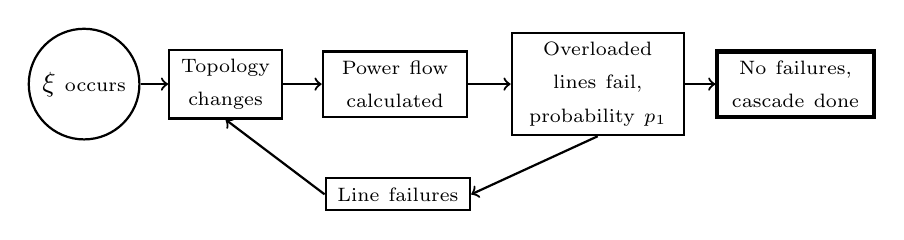
\begin{tikzpicture}
\draw [->,thick] (1,1) node[anchor=east, circle, draw]{$\xi$ \scriptsize occurs}
-- (1.35,1) node(TC)[anchor=west,text width=1.2cm,text centered,  rectangle, draw]{\scriptsize Topology changes};
\draw[->,thick] (TC)
--(3.3,1) node(PF)[anchor=west,text width=1.6cm,text centered, rectangle,draw]{\scriptsize Power flow calculated};
\draw[->,thick] (PF)
--(5.7,1) node(F)[anchor=west,text width=1.95cm, text centered, rectangle, draw]{\scriptsize Overloaded lines fail, probability $p_1$};
\draw[->,thick] (F)
--(8.3,1) node(DN)[anchor=west,text width=1.75cm, text centered,rectangle,draw,line width=1.5pt]{\scriptsize No failures, cascade done};
\draw[->,thick] (F.south)
--(5.2,-.4) node(LF)[anchor=east,text width=1.6cm, text centered, rectangle, draw]{\scriptsize Line failures };
\draw[->,thick] (LF.west)
-- (TC.south);

\end{tikzpicture} 
\caption{OPA simulation of a cascading power failure}
  \label{fig:cascade}
\end{figure}


The OPA model of the cascade process begins with an exogenous event, $\xi$, that effects the topology of the grid.  In their initial version, $\xi$ were the branches that randomly failed in an independent and identically distributed (I.I.D) manner, a Bernoulli trial with probability $p_0$.  Moments after the failure, the power flows are rerouted through the new topology based on the laws of physics.  In a longer time frame, it is possible for operators to take actions such as load shed and generator redispatch.  The resulting loading on the transmission lines is evaluated.  Their model then failed overloaded transmission lines with a Bernoulli trial with probability $p_1$ between  0.1 and 1.  After all overloaded lines are evaluated, a transition is made to the next stage.  Either there are no more failures, in which case the cascade is over, or more branch elements have failed, the topology changes, and the operator is allowed to take recourse.  This process repeats until the system is stable and no failures occur.  Figure \ref{fig:cascade-example} shows a visual example of the cascading process.

For a given grid $\cG$ and initial demand $d_0$
\begin{description}\label{fast_opa}
\item[ Initial $ \xi $ ]  For $e=1,...,n_e$, draw $\omega$ from $U[0,1]$ and if $\omega \le p_0$, line $e$ fails.
\item[ ] \hspace{35px} \vdots 
\item[ Stage $m$ ]  Calculate the power flows $f_{m}$, a column containing the branch flows for all edges in $\cE$, by using DC power flow equations with demand vector $d_m$. 

For $e=1,...,n_e$, if branch flow $f_{em} \ge U_{em}$, draw $\omega$ from $U[0,1]]$ and if $\omega \le p_1$, line $e$ fails.
\end{description}


%\documentclass{standalone}
%\begin{document}

\def \sc     { .65 }
\def \lw     { 1.25pt }

\begin{figure}
\centering
\begin{subfigure}[b]{.46\linewidth}
\begin{tikzpicture}[line width=\lw,scale=\sc]

\node[circle,fill=blue!20] (one) at (3,0) {\small 1};
\node[circle,fill=red!20] (two) at (5,0) {\small 2};
\node[rectangle,fill=green!20] (three) at (7,1) {\small 3};
\node[rectangle,fill=green!20] (four) at (5,1.75) {\small 4};
\node[rectangle,fill=green!20] (five) at (3,1.75) {\small 5};
\node[circle,fill=red!20] (six) at (2,3) {\small 6};
\node[rectangle,fill=green!20] (seven) at (5,3) {\small 7};
\node[circle,fill=red!20] (eight) at (3.85,3.45) {\small 8};
\node[rectangle,fill=green!20] (nine) at (7,3) {\small 9};
\node[rectangle,fill=green!20] (ten) at (5.85,4.1) {\small 10};
\node[rectangle,fill=green!20] (eleven) at (3.75,5) {\small 11};
\node[rectangle,fill=green!20] (twelve) at (2.35,5) {\small 12};
\node[rectangle,fill=green!20] (thirteen) at (.81,4.2) {\small 13};
\node[rectangle,fill=green!20] (fourteen) at (4,6) {\small 14};


\draw (one) -- (two) ;
\draw (one) -- (five);
\draw (two) -- (three) ; 
\draw (two) -- (four) ; 
\draw (two) -- (five) ; 
\draw (three) -- (four) ; 
\draw[red] (four) -- (five) ; 
\draw (four) -- (seven);
\draw (four) -- (nine);
\draw (five) -- (six) ; 
\draw (six) -- (eleven) ; 
\draw (six) -- (twelve) ; 
\draw (six) -- (thirteen) ; 
\draw (seven) -- (eight) ; 
\draw (seven) -- (nine) ; 
\draw (nine) -- (ten) ; 
\draw (nine) .. controls +(up:1.2cm) .. (fourteen) ;
\draw[red] (ten) -- (eleven); 
%\draw[red] (eleven) -- (twelve); 
\draw[red] (twelve) -- (thirteen);
\draw (thirteen) .. controls +(up:1.2cm) .. (fourteen) ; 
\end{tikzpicture}
\caption{Initial Event: The three red lines are outaged and the power flow redistributes.}
\end{subfigure}
\begin{subfigure}[b]{.46\linewidth}
\begin{tikzpicture}[line width=\lw,scale=\sc]

\node[circle,fill=blue!20] (one) at (3,0) {\small 1};
\node[circle,fill=red!20] (two) at (5,0) {\small 2};
\node[rectangle,fill=green!20] (three) at (7,1) {\small 3};
\node[rectangle,fill=green!20] (four) at (5,1.75) {\small 4};
\node[rectangle,fill=green!20] (five) at (3,1.75) {\small 5};
\node[circle,fill=red!20] (six) at (2,3) {\small 6};
\node[rectangle,fill=green!20] (seven) at (5,3) {\small 7};
\node[circle,fill=red!20] (eight) at (3.85,3.45) {\small 8};
\node[rectangle,fill=green!20] (nine) at (7,3) {\small 9};
\node[rectangle,fill=green!20] (ten) at (5.85,4.1) {\small 10};
\node[rectangle,fill=green!20] (eleven) at (3.75,5) {\small 11};
\node[rectangle,fill=green!20] (twelve) at (2.35,5) {\small 12};
\node[rectangle,fill=green!20] (thirteen) at (.81,4.2) {\small 13};
\node[rectangle,fill=green!20] (fourteen) at (4,6) {\small 14};

\draw[red] (one) -- (two) ;
\draw (one) -- (five);
\draw (two) -- (three) ; 
\draw[red] (two) -- (four) ; 
\draw (two) -- (five) ; 
\draw[red] (three) -- (four) ; 
%\draw (four) -- (five) ; 
\draw (four) -- (seven);
\draw (four) -- (nine);
\draw (five) -- (six) ; 
\draw (six) -- (eleven) ; 
\draw (six) -- (twelve) ; 
\draw (six) -- (thirteen) ; 
\draw (seven) -- (eight) ; 
\draw (seven) -- (nine) ; 
\draw (nine) -- (ten) ; 
\draw (nine) .. controls +(up:1.2cm) .. (fourteen) ;
%\draw (ten) -- (eleven); 
%\draw (twelve) -- (thirteen);
\draw (thirteen) .. controls +(up:1.2cm) .. (fourteen) ; 
\end{tikzpicture}
\caption{Stage 1: Lines 1-2, 2-4, and 3-4 are overloaded. Lines 1-2 and 3-4 fail, but line 2-4 remains in operation at an overloaded state. }

\end{subfigure}
\begin{subfigure}[b]{.46\linewidth}

\begin{tikzpicture}[line width=\lw,scale=\sc]

\node[circle,fill=blue!20] (one) at (3,0) {\small 1};
\node[circle,fill=red!20] (two) at (5,0) {\small 2};
\node[rectangle,fill=green!20] (three) at (7,1) {\small 3};
\node[rectangle,fill=green!20] (four) at (5,1.75) {\small 4};
\node[rectangle,fill=green!20] (five) at (3,1.75) {\small 5};
\node[circle,fill=red!20] (six) at (2,3) {\small 6};
\node[rectangle,fill=green!20] (seven) at (5,3) {\small 7};
\node[circle,fill=red!20] (eight) at (3.85,3.45) {\small 8};
\node[rectangle,fill=green!20] (nine) at (7,3) {\small 9};
\node[rectangle,fill=green!20] (ten) at (5.85,4.1) {\small 10};
\node[rectangle,fill=green!20] (eleven) at (3.75,5) {\small 11};
\node[rectangle,fill=green!20] (twelve) at (2.35,5) {\small 12};
\node[rectangle,fill=green!20] (thirteen) at (.81,4.2) {\small 13};
\node[rectangle,fill=green!20] (fourteen) at (4,6) {\small 14};

%\draw[red] (one) -- (two) ;
\draw (one) -- (five);
\draw (two) -- (three) ; 
\draw[red] (two) -- (four) ; 
\draw[red] (two) -- (five) ; 
%\draw[red] (three) -- (four) ; 
%\draw (four) -- (five) ; 
\draw (four) -- (seven);
\draw (four) -- (nine);
\draw (five) -- (six) ; 
\draw (six) -- (eleven) ; 
\draw (six) -- (twelve) ; 
\draw[red] (six) -- (thirteen) ; 
\draw (seven) -- (eight) ; 
\draw[red] (seven) -- (nine) ; 
\draw (nine) -- (ten) ; 
\draw (nine) .. controls +(up:1.2cm) .. (fourteen) ;
%\draw (ten) -- (eleven); 
%\draw (twelve) -- (thirteen);
\draw (thirteen) .. controls +(up:1.2cm) .. (fourteen) ; 
\end{tikzpicture}
\caption{Stage 2: On the new topology, lines 2-5, 6-13, and 7-9 become overloaded.  The cascade progresses by outaging lines 2-4 and 7-9.}
\end{subfigure}
\begin{subfigure}[b]{.46\linewidth}
\begin{tikzpicture}[line width=\lw,scale=\sc]


\node[circle,fill=blue!20] (one) at (3,0) {\small 1};
\node[circle,fill=red!20] (two) at (5,0) {\small 2};
\node[rectangle,fill=green!20] (three) at (7,1) {\small 3};
\node[rectangle,fill=green!20] (four) at (5,1.75) {\small 4};
\node[rectangle,fill=green!20] (five) at (3,1.75) {\small 5};
\node[circle,fill=red!20] (six) at (2,3) {\small 6};
\node[rectangle,fill=green!20] (seven) at (5,3) {\small 7};
\node[circle,fill=red!20] (eight) at (3.85,3.45) {\small 8};
\node[rectangle,fill=green!20] (nine) at (7,3) {\small 9};
\node[rectangle,fill=green!20] (ten) at (5.85,4.1) {\small 10};
\node[rectangle,fill=green!20] (eleven) at (3.75,5) {\small 11};
\node[rectangle,fill=green!20] (twelve) at (2.35,5) {\small 12};
\node[rectangle,fill=green!20] (thirteen) at (.81,4.2) {\small 13};
\node[rectangle,fill=green!20] (fourteen) at (4,6) {\small 14};

%\draw[red] (one) -- (two) ;
\draw (one) -- (five);
\draw (two) -- (three) ; 
%\draw[red] (two) -- (four) ; 
\draw[red] (two) -- (five) ; 
%\draw[red] (three) -- (four) ; 
%\draw (four) -- (five) ; 
\draw[red] (four) -- (seven);
\draw[red] (four) -- (nine);
\draw (five) -- (six) ; 
\draw (six) -- (eleven) ; 
\draw (six) -- (twelve) ; 
\draw[red] (six) -- (thirteen) ; 
\draw (seven) -- (eight) ; 
%\draw[red] (seven) -- (nine) ; 
\draw (nine) -- (ten) ; 
\draw (nine) .. controls +(up:1.2cm) .. (fourteen) ;
%\draw (ten) -- (eleven); 
%\draw (twelve) -- (thirteen);
\draw[red] (thirteen) .. controls +(up:1.2cm) .. (fourteen) ; 
\end{tikzpicture}
\caption{Stage 3: This has the effect of routing all power destined for load 8 through the north passage. Lines 13-14, 4-7, and 4-9 are outaged along the path. }
\end{subfigure}

\begin{subfigure}[b]{.46\linewidth}
\begin{tikzpicture}[line width=\lw,scale=\sc]


\node[circle,fill=blue!20] (one) at (3,0) {\small 1};
\node[circle,fill=red!20] (two) at (5,0) {\small 2};
\node[rectangle,fill=green!20] (three) at (7,1) {\small 3};
\node[rectangle,fill=green!20] (four) at (5,1.75) {\small 4};
\node[rectangle,fill=green!20] (five) at (3,1.75) {\small 5};
\node[circle,fill=red!20] (six) at (2,3) {\small 6};
\node[rectangle,fill=green!20] (seven) at (5,3) {\small 7};
\node[circle,fill=red!20] (eight) at (3.85,3.45) {\small 8};
\node[rectangle,fill=green!20] (nine) at (7,3) {\small 9};
\node[rectangle,fill=green!20] (ten) at (5.85,4.1) {\small 10};
\node[rectangle,fill=green!20] (eleven) at (3.75,5) {\small 11};
\node[rectangle,fill=green!20] (twelve) at (2.35,5) {\small 12};
\node[rectangle,fill=green!20] (thirteen) at (.81,4.2) {\small 13};
\node[rectangle,fill=green!20] (fourteen) at (4,6) {\small 14};


%\draw[red] (one) -- (two) ;
\draw (one) -- (five);
\draw (two) -- (three) ; 
%\draw[red] (two) -- (four) ; 
\draw[red] (two) -- (five) ; 
%\draw[red] (three) -- (four) ; 
%\draw (four) -- (five) ; 
%\draw (four) -- (seven);
%\draw (four) -- (nine);
\draw (five) -- (six) ; 
\draw (six) -- (eleven) ; 
\draw (six) -- (twelve) ; 
\draw (six) -- (thirteen) ; 
\draw (seven) -- (eight) ; 
%\draw[red] (seven) -- (nine) ; 
\draw (nine) -- (ten) ; 
\draw (nine) .. controls +(up:1.2cm) .. (fourteen) ;
%\draw (ten) -- (eleven); 
%\draw (twelve) -- (thirteen);
%\draw (thirteen) .. controls +(up:1.2cm) .. (fourteen) ; 
\end{tikzpicture}
\caption{Stage 4:  Finally, line 2-5 that is still overloaded is outaged. }
\end{subfigure}
\begin{subfigure}[b]{.46\linewidth}
\begin{tikzpicture}[line width=\lw,scale=\sc]


\node[circle,fill=blue!20] (one) at (3,0) {\small 1};
\node[circle,fill=red!20] (two) at (5,0) {\small 2};
\node[rectangle,fill=green!20] (three) at (7,1) {\small 3};
\node[rectangle,fill=green!20] (four) at (5,1.75) {\small 4};
\node[rectangle,fill=green!20] (five) at (3,1.75) {\small 5};
\node[circle,fill=red!20] (six) at (2,3) {\small 6};
\node[rectangle,fill=green!20] (seven) at (5,3) {\small 7};
\node[circle,fill=red!20] (eight) at (3.85,3.45) {\small 8};
\node[rectangle,fill=green!20] (nine) at (7,3) {\small 9};
\node[rectangle,fill=green!20] (ten) at (5.85,4.1) {\small 10};
\node[rectangle,fill=green!20] (eleven) at (3.75,5) {\small 11};
\node[rectangle,fill=green!20] (twelve) at (2.35,5) {\small 12};
\node[rectangle,fill=green!20] (thirteen) at (.81,4.2) {\small 13};
\node[rectangle,fill=green!20] (fourteen) at (4,6) {\small 14};


%\draw[red] (one) -- (two) ;
\draw (one) -- (five);
\draw (two) -- (three) ; 
%\draw (two) -- (four) ; 
%\draw[red] (two) -- (five) ; 
%\draw[red] (three) -- (four) ; 
%\draw (four) -- (five) ; 
%\draw (four) -- (seven);
%\draw (four) -- (nine);
\draw (five) -- (six) ; 
\draw (six) -- (eleven) ; 
\draw (six) -- (twelve) ; 
\draw (six) -- (thirteen) ; 
\draw (seven) -- (eight) ; 
%\draw[red] (seven) -- (nine) ; 
\draw (nine) -- (ten) ; 
\draw (nine) .. controls +(up:1.2cm) .. (fourteen) ;
%\draw (ten) -- (eleven); 
%\draw (twelve) -- (thirteen);
%\draw (thirteen) .. controls +(up:1.2cm) .. (fourteen) ; 
\end{tikzpicture}
\caption{Stage 5:  The system stabilizes into islands with generator 1 serving load 6.  However, loads 2 and 8 are out of service.}
\end{subfigure}
\caption[An example of the OPA cascading sequency]{ \label{fig:cascade-example} \small An example of a cascading power failure. Node 1 is a generator and nodes 2, 6, and 8 are loads.}
\end{figure}

%\end{document}


\subsubsection{Dynamic Equilibrium}

These opposing forces eventually find an equilibrium.  The equilibrium tends to be near critical points, which are points that have maximum power flow through the network for the nominal system capacity.  The system self-organizes toward these points, which maximize efficiency of its assets.  When the system approaches these critical points, the power flow becomes limited due to two possible causes:
\begin{itemize}
\item The power flows are limited due to transmission line constraints.  This type of critical point has larger blackouts, but happens less frequently.  In addition, the blackouts typically have  multiple lines tripping.
\item The power flows are limited due to generation capacity.  This results in frequent blackouts, but of smaller size.
\end{itemize}
However, it is also possible to be in an operating regime which is close to both types of critical points simultaneously.  When this is the case, blackouts of all sizes occur.  While this operating regime may not be good from a reliability standpoint, it has the desirable characteristic of being able to deliver the maximum power for the system.   That is, when these two points are balanced, the system is capable of maximum throughput from its generators to its loads with minimal excess capacity.  This is important from an economic perspective and a critical reason the system self-organizes to these types of points.  This type of point tends to be the cheapest way to supply all the loads with power, while statisfying the minimum system reliability standards.

\subsubsection{Additional Complexities}

The OPA model can be extended to include many additional complexities.  It is always a balance of how much resources you have to solve the problem and the amount of resolution you need in the solution.  The base OPA model is easy and fast to replicate, however by trying to gain increased resolution in the output, the model becomes increasingly complex and difficult to solve in a timely manner.

In related work, Chen et. al. \cite{chen_2005} find many similar conclusions to the OPA model by using an extension which included a hidden failure model.  A hidden failure is undectable in normal operations, but as the system becomes disturbed, a relay may incorrectly trip.  These protective relays are in operation to protect the line from overloads and disconnect it from the system.  This work introduces a loading dependent failure model that trips neighboring lines and nearby components fail.  This hidden failure is exposed the first time a disturbance nearby occurs and if it doesn't fail then, it is assumed to be properly operating and future disturbances will not undergo this hidden failure mechanism.  The probability of these happening in the real world are non-negligble according to NERC data \cite{nerc_dawg}.  

This work displays many similar results to the OPA papers.  First, the power law behavior near critical loading can be seen by varying the system loading levels.  They find that by increasing spinning reserves the risk of big blackouts is greatly reduced.  The blackout size distribution tends toward an exponential distribution as reserve levels are increased.  By lowering the hidden failure rate, the system becomes more robust and larger blackouts become less likely.  Finally, they note that prompt control actions can reduce the risk of big disturbances.  While all of these results seem fairly straightforward, it points to the fact that the important aspects of the cascading process are being modeled and the effects are similar to what would happen in the real world.

Bienstock made several modifications \cite{bienstock_2011} to the original OPA model in order to remove some undesirable effects of the simulation, notably the erratic behavior of its output under small changes in the input.  To do this, he introduced the concept of memory to the system.  In order to see if a line is in or near an overloaded state, it uses a running time average of the current state and previous states.
\begin{equation}
\tilde{f}_{et} = \alpha f_{et} + (1-\alpha) \tilde{f}_{e\rho(t)}
\end{equation} 
Here, $f_{et}$ represents the power flow on edge $e$ at time $t$.  Then, $\tilde{f}_{et}$ is used in the overload and line failure calculations.

In addition to including a memory, he also smoothed out the definition of an overloaded line by creating a step in between normal and overloaded states in which the failure probability was more than nominal but less than in the overloaded state.  Using $0 \le \epsilon \le 1$, for edge $e$, the following failure model smooths the effects of overloaded lines failing.
\begin{align}
\tilde{f}_{et} \ge (1+\epsilon) U_{et}			&	\hspace{10pt} \mbox{The line fails with certainty} 	\\
(1-\epsilon) U_{et} < \tilde{f}_{et} < (1+\epsilon) U_{et}	&	\hspace{10pt} \mbox{The line fails with probability }\frac{1}{2} 	\\
\tilde{f}_{et} \le (1-\epsilon) U_{et}			&	\hspace{10pt} \mbox{The line remains in operation} 
\end{align}

An AC power blackout model was developed at the University of Manchester (Manchester Model) by Nedic \cite{nedic_2006} and the original OPA authors.  This model is able to represent real world disturbances more accurately by using the full non-linear model that describes power flow.  This gives resolution into areas for generator instability, under-frequency load shedding, redispatch of active and reactive sources, and emergency load shedding.  The model has both automated control systems and operator recourse.  This model was used in OPA criticality works by Mei et. al. \cite{mei_2006}, including one with mechanisms using voltage stability margins \cite{mei_2008}.  However, the additional complexity comes at the cost of having to solve a nonlinear program and the loss of convergence gaurantees.  This is all done in order to represent something that is a companion to, but not the main driver of the cascading process (according to the Northeast outage working group, the main driver was angle instability not voltage instability).

Mei {\it et. al.} have worked to improve the accuracy of OPA by increasing the level of detail \cite{mei_2009}.  In the fast dynamics, along with protective relays being modeled as hidden failures, they included a failure mechanism for the operational dispatch center that is responsible for generator redispatch.  In addition, they used a failure model where an underloaded line is failed with probability $p_1 \left( f_e/U_e \right)^N$, with $N=10$.  For the slow dynamics, they added a step that models a planning department by increasing the capacity of lines which have a loading rate $\left( f_{e}/ U_{e}  \right)$ greater than a set point.  

In 2013, Qi {\it et. al.} extended this model to include slow dynamics of vegetation growth and management as well as differential equations representing line heating \cite{qi_2013}.  Neglecting spatial variation and heating/cooling effects from   the environment, they model line temperature by a differential equation
\begin{equation}
\frac{dT(t)}{dt} = \alpha I^2 - \nu (T(t) - T_0)
\end{equation}
where $T(t)$ is the line temperature at $t$, $I$ current, $T_0$ initial temperature, and $\alpha$ and $\nu$ are calculated parameters.  This can be solved by assuming constant branch flow, $f$, to calculate the temperature over time
\begin{equation}
T(t) = e^{-\nu t}\left( T_0 - T_e(f) \right) + T_e(f)
\end{equation}
which can be used to find the final equilibrium temperature, $T_e(f)$ (a function of its constant power flow $f$ on the line), and time until a given temperature.  Using the calculated temperature, the horizontal span, and an elongation parameter, the line sag distance can be calculated.  When the minimum distance between lines and vegetation passes a breakpoint based on transmission line characteristics such as operational voltage, the line will fail.  They model the vegetation with a daily growth rate model and include a managment simulation in which they identify future potential hazards and cut down trees over time.  The statistical analysis of their model agreed well with historical data in China.


\subsection{Power Flow Review}
In order to run the OPA simulation of cascading failures, the ability to calculate power flows on the system is critical.  To model a balanced, three phase power flows, in full resolution we need to model complex power.  The alternating current of the power system can be represented by sine or cosine waves.  A three phase power system has three lines for each transmission element and each line has a wave that is out of phase with the other two.  Using one wave as a reference, the other phases attempt to be 120 degrees behind reference and 120 degrees ahead of reference.  This improves the efficiency and quality of power for loads over a 2 line system as well as not requiring an excessive number of lines for each transmission element.  

Complex power has both real and reactive parts.  Alternating currents  on a circuit affect components of energy storage such as inductors (changing the current as opposed by a voltage)  or capacitors (store electrical charge).  Over one full cycle of the electricity changing direction, across any individual element there can be real power transferred.  However, there is also power which is stored and released within one cycle and the net energy transfer of this power is 0.  This is called reactive power and is modelled as the imaginary component of complex power.  




In a balanced three phase system, at every vertex $i$, we have
\begin{equation}
S_i = P_i + j Q_i = V_i I_i^*
\end{equation}
where $P$ is real power, $Q$ is reactive power, $V_i$ is complex voltage, and $I_i^*$ is the complex conjugate of current.  In addition, with Kirchoff's Current Law, we have $I_i = \sum_{k=1}^n Y_{ik} V_k$, where $Y$ is the admittance bus matrix.  The admittance is the inverse of imdedence, that is
\begin{equation}
Y = G + j B = 1/Z = 1/(R + jX) 
\end{equation}
where $B$, the imaginary part of admittance, is susceptance and $X$, the imaginary part of impedence, is reactance.  Now we have that the complex power at every vertex $i$ is
\begin{equation}
S_i^* = P_i - j Q_i = V_i^* \sum_{k=1}^n Y_{ik} V_k
\end{equation}
By converting these into rectangular coordinates, we get two equations for each bus
\begin{align}
P_i = \sum_{k=1}^n |V_i| |V_k| \left[ G_{ik} \cos (\theta_i - \theta_k) + B_{ik} \sin (\theta_i - \theta_k) \right]  \label{activepower}\\
Q_i = \sum_{k=1}^n |V_i| |V_k| \left[ G_{ik} \sin (\theta_i - \theta_k) - B_{ik} \cos (\theta_i - \theta_k) \right] 
\end{align}

For each bus, in addition to $P_i$ and $Q_i$,  we have its voltage $|V_i|$ and its phase angle $\theta_i$.  So, we have $4 n_v$ variables and $2 n_v$ equations.  By supplying the value to $2 n_v$ variables and defining a slack bus, we can find unique values for the remaining $2n_v - 1 $ variables.  Depending on the type of bus, different variables are supplied.  If it is a generator, both $P$  and $V$ are supplied.  A load is defined by a $P$ and $Q$.  The slack bus is a generator in which the phase angle is set to 0.  The phase angle $\theta$ and reactive power production $Q$ are found for each generator and the phase angle $\theta$ and the voltage $|V|$ are found for the loads.


%\endnote{\textbf{Electrical Information}

Complex power has both real and reactive parts.  Alternating currents  on a circuit affect components of energy storage such as inductors (changing the current as opposed by a voltage)  or capacitors (store electrical charge).  Over one full cycle of the electricity changing direction, across any individual element there can be real power transferred.  However, there is also power which is stored and released within one cycle and the net energy transfer of this power is 0.  This is called reactive power and is modelled as the imaginary component of complex power.  Let $S_i$ be the complex power inject at some bus on the grid, that is
\begin{equation}
S_i = P_i + j Q_i = V_i I_i^*
\end{equation}
where $P$ is real power, $Q$ is reactive power, $V_i$ is complex voltage, and $I_i^*$ is the complex conjugate of current.  
	
To model a transmission line, the characteristic impedence is used.  At any point, there is complex current I, in each individual line in the transmission element.  Also, there is a complex voltage V difference between the lines.  The characteristic impedence (generalization of Ohm's Law) is then
\begin{equation} \label{impedence}
V/I = Z_0
\end{equation}

Here is a phasor representation of complex voltage $V_i = | V_i | e^{i (\omega t + \delta_i) }$, where the real voltage would be Re[$V_i$]$=\cos (\omega t + \delta_i)$.  Now, by modeling \ref{impedence} in phasor notation, we have 
\begin{equation}
 | V_i | e^{j (\omega t + \delta_V) } = | I_i | e^{j (\omega t + \delta_I) }  | Z_i | e^{j ( \delta_Z) } = |I||Z|e^{j (\omega t + \delta_I + \delta_Z)}
\end{equation}
For this equation to hold at all times $t$, we know that this must hold $\delta_V = \delta_I + \delta_Z$.  When an element has $\delta_Z = 0$, the current and voltage are exactly in phase and it is a purely resistive load with no reactive production or absorption. 

The lines can be modelled using a pi model (schematic diagram looks like $\pi$), which uses line parameters of resistance $R$, inductance $L$, conductance $G$, and capacitance $C$. 
\begin{equation}
Z_0 = \sqrt{  \frac{R+j \omega L}{G+j\omega C} }
\end{equation}
The system angular frequency is $\omega = 2 \pi f$, where $f$ is frequency here.  

If a transmission element is loaded at its surge impedence loading, it neither creates nor consumes reactive power.  This level is defined by 
\begin{equation}
SIL = V_{LL}^2 / Z_0
\end{equation}
Where $V_{LL}$ is the line to line voltage.  When a transmission line is at a level below this, it will supply reactive power and raise system voltages.  When the loading is above this level, the transmission line consumes reactive power, depressing voltages.
} \endnote{\textbf{Balanced Three Phase Power Flow}

In a balanced three phase system, at every vertex $i$, we have
\begin{equation}
S_i = P_i + j Q_i = V_i I_i^*
\end{equation}
In addition, with $KCL$, we have $I_i = \sum_{k=1}^n Y_{ik} V_k$, where $Y$ is the admittance bus matrix.  The admittance is the inverse of imdedence, that is
\begin{equation}
Y = G + j B = 1/Z = 1/(R + jX) 
\end{equation}
where $B$, the imaginary part of admittance, is susceptance and $X$, the imaginary part of impedence, is reactance.  Now we have that the complex power at every vertex $i$ is
\begin{equation}
S_i^* = P_i - j Q_i = V_i^* \sum_{k=1}^n Y_{ik} V_k
\end{equation}
By converting these into rectangular coordinates, we get two equations for each bus
\begin{align} \label{ac-pf}
P_i = \sum_{k=1}^n |V_i| |V_k| \left[ G_{ik} \cos (\delta_i - \delta_k) + B_{ik} \sin (\delta_i - \delta_k) \right]  \\
Q_i = \sum_{k=1}^n |V_i| |V_k| \left[ G_{ik} \sin (\delta_i - \delta_k) - B_{ik} \cos (\delta_i - \delta_k) \right]  
\end{align}

For each bus, in addition to $P_i$ and $Q_i$,  we have its voltage $|V_i|$ and its phase angle $\delta_i$.  So, we have $4 n_v$ variables and $2 n_v$ equations.  By supplying the value to $2 n_v$ variables and defining a slack bus, we can find unique values for the remaining $2n_v - 1 $ variables.  Depending on the type of bus, different variables are supplied.  If it is a generator, both $P$  and $V$ are supplied.  A load is defined by a $P$ and $Q$.  The slack bus is a generator in which the phase angle is set to 0.  The phase angle $\delta$ and reactive power production $Q$ are found for each generator and the phase angle $\delta$ and the voltage $|V|$ are found for the loads.}  
The non-linear AC power flow equations model the net power and reactive power injects as well as voltage and phase angle at each vertex of the power system.  A few simplifying assumptions are made to allow the equations to become linear for the DC (decoupled) power flow equations.  Then, using the DC power flow model, basic economic dispatch and unit commitment models are shown.  
%Finally, some pseudo-topological measures will be reviewed that will be useful in the optimization process.

\subsubsection{Decoupled Power Flow}
This model makes assumptions such as lossless lines, small voltage angle differences, and a flat voltage profile.  This is a common simplifying model which is used routinely in economic and reliability analysis of power systems.  A flat voltage profile implies that $\forall i \in \cV$, we have $V_i = 1$.  Small voltage angle difference in conjunction with sine and cosine give the following approximations
\begin{align}
\cos(\theta_i - \theta_j) &\approx 1	\\
\sin(\theta_i-\theta_j) & \approx \theta_i - \theta_j
\end{align}
In addition, since these lines are lossless, $R$ and $G$ are 0.  Using this approximations, \Cref{activepower} becomes
\begin{equation}	\displaystyle
\theta_{i} - \theta_{j} = X_{e} f_{e}			\hspace{27px}	\forall e=(i,j) \mbox{ s.t. } e \in \cE   \label{pf2}
\end{equation}
where $X_e = B_{ij}^{-1}$.  We also have conservation of energy at each bus in the network, implying that the sum of generation and demand is equal to net flow into the transmission network, given by
\begin{equation}
\sum_{e \in \cE | e=(i,j)}{f_{e}} = g_{i} -d_{i} \hspace{17px}   \forall i \in \cV.   \label{pf1}
\end{equation}
When a line has failed, the power flow has obviously dropped to 0, that is $f_e = 0$.  In addition,  since there is no link between the phase angles, \Cref{pf2} should no longer be enforced.

\subsubsection{Economic Dispatch}
To clear the electricity market at a single point in time, a least cost dispatch model is used.  This model takes bids from generators, a known demand, as well as transmission and ramping constraints and finds a set of generator outputs that meet the demand at least cost.  Using a quadratic cost function for the generators (this cost function can be thought of as a bid from generators which includes the profit the generator would like to make for each marginal unit of production), the least cost dispatch Model (\ref{leastcostdispatch}) can be built. 

The following model is a quadratic program with linear constraints.  The objective function is to minimize the cost of generation.  Typical least cost dispatch and unit commitment models make various assumptions to allow for linear constraints versus the physical nonlinear constraints to which the power system is subject.  Model (\ref{leastcostdispatch}) is the most basic least cost dispatch model, which could be used for clearing the real-time market.  Models in use can have extensions such as ``$N-1$ constraints", which are reliability and security requirements.

\begin{subequations}
\begin{align}
 \min \sum_i c^2_i x_i^2 &+ c^1_i x_i	+ W_i(\tilde{d} - d_i)&	\\
x_i - d_i &= \sum_j y_{ij}	&	\forall i \in \cI 	\\
X_{e} f_{e} &= \theta_i - \theta_j & \forall e=(i,j) \in \cE \\
x_i  &\in \left[ G_i^- , G_i^+ \right]		&	\forall i \in \cI 	\\
y_{e} &\in \left[ -U_{e}, U_{e} \right]	&	\forall e=(i,j) \in \cE 
\end{align}
\label{leastcostdispatch}
\end{subequations}

Here, $c^2_i x_i^2 + c^1_i x_i$ can be seen as the cost function for the generator at node $i$ and $W_i(\tilde{d} - d_i)$ is the cost for shedding load.  The generator is bounded between a maximum $G_i^+$ and minimum $G_i^-$ that represent its ramping rate and other physical limits over a specific time interval.    If node $i$ cannot generate power, then $G_i^+=G_i^-=0$.

The day-ahead market uses unit commitment models.  This model has power flow equations for each time $t$ in the day $t \in \cT$.  These are integer programs due to the introduction of binary variables $w_{it}$, which take on the value 1 if the generator is switched on and 0 if the generator is off.  The following logical constraint enforces this by
\begin{equation}
w_{it} g_i^- \le g_{it} \le w_{it} g_i^+.
\end{equation}
The cost function can then include a fixed cost for operating a generator, such as increased staff during operation.  This cost is not dependent on the level of production but rather if the plant is in an on or off state.  The cost function for each node $i$ and time period $t$ is
\begin{equation}
c^2 x_{it}^2 + c^1_i x_{it} + c^0_i w_{it}
\end{equation}
This subproblem is used in a full-day model in which the power flow problem is solved for each time period, while remaining feasible with respect to ramping rates and on and off times for generators.





\section{Multi-Stage Stochastic Programming}

We use the framework of stochastic programming to model the dynamics of cascading power failure.  Each stage represents an epoch at which one or more lines fail based upon their loading.  The multi-stage stochastic program as a large mixed-integer linear program can be approximated.

\subsection*{Mixed-Integer Program}
The mixed-integer formulation of cascading power failures uses binary variables to model line availability for stages in the cascade.  In addition to these extra variables, some input parameters are needed to formulate the problem.  First, the number of stages, $n_T$, for the cascade needs to be decided.  If large blackouts are of interest, this number should be large enough to not exclude the worst-case scenarios.  Also, the number of outcomes $n_0$ at each node  of the scenario tree needs to be decided.  These outcomes represent the decision-dependent uncertainty.  The size of the problem is related to the size of the stochastic tree, which is $n_o^{ n_T }$.  As the subproblem is difficult, the computational complexity of this problem increases rapidly with the number of outcomes and stages.

\begin{figure}
\centering
\documentclass{standalone}
\usepackage{tikz}
\begin{document}
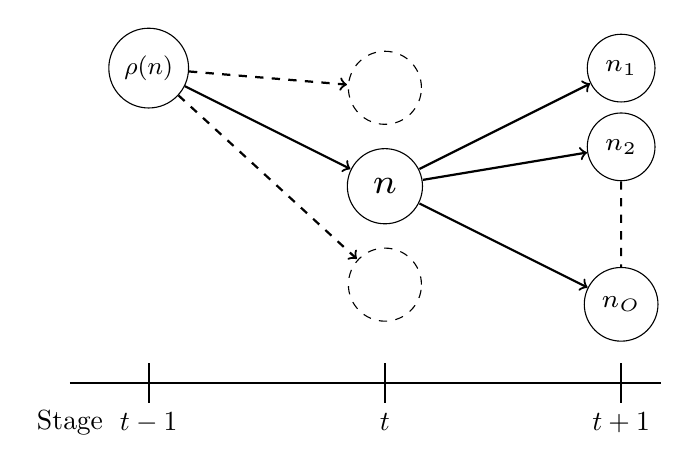
\begin{tikzpicture}

\draw (-1,2.5) node(RHO)[circle,draw]{\small $\rho(n)$ };
\draw (2,2.25) node(NUP)[circle,dashed,scale=2.8,draw]{ };
\draw (2,1) node(N)[circle,scale=1.8,draw]{\scriptsize $n$ };
\draw (2,-.25) node(NDOWN)[circle,dashed,scale=2.8,draw]{ };
\draw (5,2.5) node(N1)[circle,scale=1.3,draw]{\scriptsize $n_1$ };
\draw (5,1.5) node(N2)[circle,scale=1.3,draw]{\scriptsize $n_2$ };
\draw (5,-.5) node(NO)[circle,scale=1.3,draw]{\scriptsize $n_O$ };

\draw[thick,dashed, ->] (RHO) -- (NUP);
\draw[thick,->] (RHO) -- (N);
\draw[thick,dashed, ->] (RHO) -- (NDOWN);
\draw[thick,->] (N) -- (N1);
\draw[thick,->] (N) -- (N2);
\draw[thick,->] (N) -- (NO);
\draw[thick,dashed] (N2) -- (NO);

\draw[thick] (-2,-1.5) -- (5.5,-1.5);
\draw[thick] (-1, -1.75) -- (-1, -1.25);
\draw[thick] (2, -1.75) -- (2, -1.25);
\draw[thick] (5, -1.75) -- (5, -1.25);

\draw(-2,-2) node {Stage};
\draw(-1,-2) node {$t-1$};
\draw(2,-2) node {$t$};
\draw(5,-2) node {$t+1$};

\end{tikzpicture} 
\end{document}

\caption{Scenario tree for Mixed-Integer Formulation}
  \label{fig:mip}
\end{figure}


\subsection{Decision Dependent Uncertainty}\label{decisiondependentuncertainty}
In order to model the decision-dependent uncertainty, a cumulative distribution function (cdf) for line failures based on loaded is needed.  This model uses a parameter, $R$, to represent the effective capacity of a line.  Scenarios are created by sampling from the cdf before formulating the MIP.  This { \it effective capacity} represents the loading of the transmission line that causes its failure, and we capture the failure of a line with a binary variable, $z$. \\

In Mixed-Integer Programming, there have been standard equations developed to model logical conditions.  We have two logical conditions that need to be modeled in order to represent this decision dependent uncertainty.  First, the condition that the line will fail if it has more power flow than its effective capacity.
\begin{align*}
\mbox{If }
		\hspace{30px}&\left| y_{e\rho(n)} \right| > R_{en}  \\
\mbox{Then }
		\hspace{30px}&z_{en} = 0
\end{align*}

To model this logic, a Big-M constraint can be used, where $M$ represents a large number defined below.
\begin{align}
	y_{e\rho(n)} - R_{en} &\le M^R_e (1-z_{en})	\label{r1}\\
	y_{e\rho(n)} + R_{en} &\ge - M^R_e (1-z_{en})	\label{r2}
\end{align}
with $M^R_{en} = U_e - R_{en}$. \\

Now, when the line is available in stage $n$, that is $z_{en} = 1$, then the line flow in the predecessor node is within the effective capacity, -$R_{en} \le f_{e\rho(n)} \le R_{en}$.		\\

The second logical condition is that when the line is unavailable, the power flow on that branch is zero and the phase angles between the two nodes are not constrained. 
\begin{align*}
\mbox{If }
		\hspace{20px}&z_{en} = 0	\\
\mbox{Then }
		\hspace{20px}&y_{en} = 0  \hspace{10px} \mbox{ and}\\
				&\theta_{in} - \theta_{jn} - X_{e}y_{en} \mbox{ is arbitrary}
\end{align*}	

This can be achieved through the following equations.
\begin{align}
-U_{e} z_{en} \le y_{en} &\le U_{e} z_{en}	\label{lf1}\\
\theta_{in} - \theta_{jn} + X_e y_{en} &\ge -M^\theta_e(1-z_{en}) \label{lf2} \\
\theta_{in} - \theta_{jn} + X_e y_{en} &\le M^\theta_e(1-z_{en})  \label{lf3}
\end{align}
with $M^\theta_e = 2 \theta_{max} + X_e U_e$.


\subsection*{Failure Density Function}
The OPA simulation uses a step function for the failure probability of a line shown in \Cref{opafail}.  We modify the effective capacity distribution to give ramp up line failure risk according to a piecewise linear function also shown in \Cref{opafail}   To approximately model this analytically, a sample from the distribution can be used to form the effective capacity of the lines.  Let $\omega_n \equiv\left[ 0, 0, 1, 0, \cdots, 1\right]$  be a vector sampled from a Bernoulli distribution and let $\alpha_n \in \R{|\cE|}$ be a vector sampled from a uniform distribution between $L_e$ and $U_e$ for each line.  Now, a line fails if $y_{ne} \ge \alpha_{ne} U_e$ and $\omega_{ne} =1$.  With this sampling, the effective capacity can be designed to incorporate this information.    
\begin{equation}
 R_{ne} = 
 \left\{ 
	\begin{array}{lr}
				\alpha_{ne} U_e & \mbox{if } \omega_{ne}=1\\
			  U_e + \epsilon & \mbox{if } \omega_{ne}=0
	\end{array}
 \right. \label{r}
\end{equation}

The resulting set of effective capacities $R$ can be represented by a cumulative distribution function. The distribution in Figure \ref{cdf} is one example of a viable line failure distribution input.  It is the result of a uniform distribution for $\alpha$ between $L$ and U and Bernoulli trial with probability $p$ for $\omega$.  


\begin{figure}
\centering
\pgfplotsset{every axis plot/.append style={line width=2pt}}
\tikzset{
every pin/.style={fill=yellow!50!white,rectangle,rounded corners=3pt,font=\tiny},
small dot/.style={fill=black,circle,scale=0.3}
}

\begin{tikzpicture}[scale=.8]
\begin{axis}[ 
	xlabel=$r$,
	ylabel=$P( R < r )$,
	title = OPA Effective Capacity,
	unbounded coords = jump,
	xtick= {0},
	ytick= {0, 1},
	extra y ticks={.5},
	extra y tick style={grid=major},
	extra y tick labels={$p$},
	extra x ticks={.575,1},
	extra x tick labels={$L$, $U$},
        xmax=1.1,
scatter/classes={
 		 a={mark=o,line width=3.5pt},%
 		 b={mark=o,line width=1pt,scale=1.75}%
		}]
	\addplot[black] coordinates { 
		(0,0)		
		(.985,0) 		
		(1,inf)		
		(1,1)		
		};	
	\addplot[black] coordinates { 
		(1.0225,1)		
		(1.5,1) };	
	
\addplot[ 
		scatter,only marks,
		scatter src=explicit symbolic]
		coordinates {  
		(0,0)		[a]
		(1,0)		[b]
		(1,.5)		[a]
		(1,1)		[b]
		};


	

\end{axis}
\end{tikzpicture}
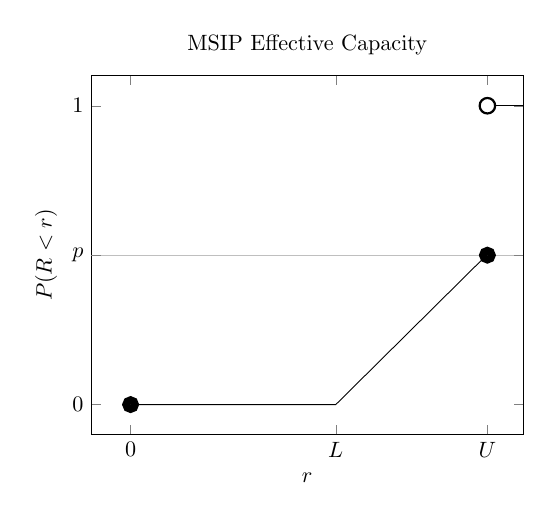
\begin{tikzpicture}[scale=.8]
\begin{axis}[ 
	xlabel=$r$,
	ylabel=$P( R < r )$,
	title = MSIP Effective Capacity,
	unbounded coords = jump,
	xtick= {0},
	ytick= {0, 1},
	extra y ticks={.5},
	extra y tick style={grid=major},
	extra y tick labels={$p$},
	extra x ticks={.575,1},
	extra x tick labels={$L$, $U$},
        xmax=1.1,
scatter/classes={
 		 a={mark=o,line width=3.5pt},%
 		 b={mark=o,line width=1pt,scale=1.75}%
		}]
	\addplot[black] coordinates { 
		(0,0)		
		(.575,0)	
		(.985,.485) 		
		(1,inf)		
		(1,1)		
		};	
	\addplot[black] coordinates { 
		(1.0225,1)		
		(1.5,1) };	
	\addplot[ 
		scatter,only marks,
		scatter src=explicit symbolic]
		coordinates {  
		(0,0)		[a]
		(1,.5)		[a]
		(1,1)		[b]
		};


	

\end{axis}
\end{tikzpicture}

\caption{ Example Effective Capacity Distributions}
\label{cdf}
\end{figure}



\subsection{Cascade Evolution}\label{feasiblecascades}
The cascading process begins with an intial exogenous event, $\xi \in \left\{ 0, 1 \right\}^{\magE}$.  This may be treated as a random vector on a probability space with sample space $\Xi$.  The following equation enforces a line failure throughout the whole cascade for all $e \in \cE$ such that $\xi=1$.

\begin{equation}
z_{en} \le 1- \xi_e . \label{xi}
\end{equation}

Now, the cascade will evolve according to the dispatch decisions chosen and the pre-sampled effective capacities of the particular lines during the various stages of the cascade.  The operators will be able to optimize the cost, which includes the cost of load shed, and are constrained to be within the following set, 
\begin{equation}
\Omega(\xi) \equiv \left\{ \left(d, x, y, z \right)  |  \mbox{ \Cref{pf1,pf2,r1,r2,lf1,lf2,lf3,r,xi}  hold } \right\} 
\end{equation}
where $d = \left[ d_0, d_1, \cdots, d_N \right]$ is the set of vectors of demand served for each node in the scenario tree.  Now, this representation of the cascading process can be used in many ways.  One example is a chance constrained model, in which the operator requires a line to be available in a certain percentage of scenarios.  Another example is to use this a sa subproblem in a larger planning model. 

\subsection{Least Cost Dispatch}
The following model is a least cost dispatch model that includes the effects from cascading failures due to a set of contingencies $\xi\in\Xi$.
\begin{subequations}
\label{leastcost}
\begin{align} \displaystyle
	{\large \mbox{min}} \hspace{10px} &  \Expect_\Xi \sum_{in} \left[ c^2_{in}  x^2_{in,m} + c^1_{in} x_{in,m}  + W_{in} (\hat{d}_{i} - d_{in,m}) \right]	\\
	&(d,x,y,z)_m  \in \Omega(\xi_m)    \hspace{20px}   \forall \xi_m \in \Xi	
\end{align}
\end{subequations}
This can be adapted to several different problems in power systems.  The main difficulty with this multi stage stochastic program is computational complexity.  The program can be calibrated in order to produce similiar load shed distributions to the OPA model, however the number of outcomes and stages in the model needs to be small or the computational hurdle becomes too large.

In order to get reliable output from the optimization routine, this model needs to be calibrated against the OPA simulation.  The primary calibration parameters are $L$ and $p$ in the line failure distribution shown in \Cref{cdf} as well as the costs for load shed, $W$, which depend upon the stage in the cascade.  The OPA simulation is a greedy algorithm, attempting to maximize demand served in the current stage without regard to the line failure consequences.  In order to capture this effect, more weight was placed on demand served in earlier stages of the cascade. \\

 The root problem used is comprised of 4 intitial outages and each outage has a scenario tree that is 4 stages long with 2 outcomes at each node.  The power system modeled is the IEEE 118 bus grid with a nominal demand of 3668 MW and around 29,600 MW in branch capacities.  The parameters chosen for the MSIP model were $p=.5$, $L =.575$.  The weights $W_s$ for the stages of the cascade were $[500, 10, .05, .0001]$, which seemed to capture the greedy behavior of the OPA simulation.  The OPA simulation used the step function failure model with $L=.99$ and $p=.5$.  The output of the simulation and MSIP formulation are shown in Table (\ref{compare}) along with the load shed distribution for initial line failures on lines $[12,14,34,111]$ in Figure (\ref{dist}). 


% Calibrate ---------------------------------------------------------


\begin{figure}
 \centering
	\begin{tikzpicture}
		\begin{axis}[xlabel=$LS$ (MW), ylabel=$P($Load Shed $> LS )$
				,legend pos=north east
				,grid=major,
				,xmin=-25,xmax=400
				,title=\mbox{Load Shed Distribution} ]


 	\addplot[black,line width=3pt] table[x=mv, y=mp] {./data/calibrate.txt};
	\addlegendentry{MSIP}
	
	\addplot[red,line width=2pt] table[x=sv, y=sp,mark=square] {./data/calibrate.txt};
	\addlegendentry{SIM}





		\end{axis}	
	\end{tikzpicture}
  \caption{Load Shed Distribution for the OPA simulation and MSIP formulation}
 \label{dist}
\end{figure}


\begin{table}
\centering
\begin{tabular}{| c | c c | c c |}
\hline
Initial	&	\multicolumn{2}{ | c | }{ SIM } & \multicolumn{2}{|c|}{MSIP} \\
Contingency	&	$\Expect [ LS ]$ & St.Dv.$ [LS]$ &	$\Expect [LS]$ & St.Dv.$ [LS]$  \\
\hline
\hline
2,12,21 &	196 & 128.1 & 184 & 112.7 \\
5,25,34, 82 &	254 & 187.1 & 160 & 69.3 \\
12,14,34,111 & 	131 &	 85.12 &	 151 &	 59.0 \\
13,24 	&	145 & 123.4 	&	123	&	84.4 \\

\hline
\end{tabular}
\caption{Comparison of Simulation and MSIP outputs}
\label{compare}
\end{table}


\section{Model Flexibility}
The primary strength of this formulation is the flexibility it has in using additional constraints and objectives to inform decision making about power systems.  All of these models can then be solved with commercial solver software without the need to develop additional specialized routines.  The first example is a chance constrained model, which enforces a probabilistic constraint on the number of line failures in any scenario. 
%\endnote{\textbf{Chance Constraint on N-k Criteria}

In this model, constraints are used to express the probability that less than a given number of lines are outaged is close to 1.  A typical case in power systems would be that the system should not go beyond 1 contingency in a large percentage of scenarios.
\begin{equation}
P\left\{\text{Line Outage} \le k \right\} \ge 1 - \epsilon
\end{equation}
This can be done by adding another binary variable for each scenario that represents whether or not that scenario has less than $k$ outages.  Then these new binary variables will be summed and constrained by the given probability.
\begin{subequations}
\begin{align}
\sum_i z_{is} &\le	M_s \hat{z_s} + | \xi_s | + k \\
\sum_s \hat{z_s} &\le \epsilon | \cS |
\end{align}
\end{subequations}
where $M_s = | \cE | - | \xi_s | - k$.  The objective of this program would be to minimize load shed as in (\ref{leastcost}) such that the power system does not lose more than $k$ branches.
}  
In this model, we constrain the probability that fewer than a given number of lines failures to be close to 1.  A typical case in power systems would be that the system should not go beyond 1 contingency in a large percentage of scenarios.
\begin{equation}
P\left\{\text{\# Line Failure} \le k \right\} \ge 1 - \epsilon
\end{equation}
This can be done by adding another binary variable for each scenario that represents whether or not that scenario has fewer than $k$ failure.  These new binary variables are summed and constrained by the given probability.
\begin{subequations}
\begin{align}
\sum_i z_{is} &\le	M_s \hat{z_s} + | \xi_s | + k \\
\sum_s \hat{z_s} &\le \epsilon | \cS |
\end{align}
\end{subequations}
where $M_s = | \cE | - | \xi_s | - k$.  The objective of this program would be to minimize load shed as in Model (\ref{leastcost}).


The second example is a redispatch model that moves to a generator configuration that is close to the original while minimizing the expected size of the cascade.
%\endnote{\textbf{Generator Redispatch}

This model tries to find an operating configuration that is within a given distance from the current operating regime and minimizes the worst case scenario outage.  The input for this model is the current operating configuration $(p_0, d_0)$ as well as a distance vector $\delta$ that represents how far each generator can move from its current output levels.  In this case, the root node of the stochastic tree will have variables that represent initial generator output levels and the child trees will be constrained from how far they can move from this.  Also, a continuous variable will be added that represents the amount of load shed in the worst case scenario.  The objective will be to minimize this worst case scenario.  
\begin{equation}
p - p_0 \le \delta
\end{equation}
\begin{equation}
l \ge \sum_i \hat{d}_i - d_{is}
\end{equation}
aim to min 
This program could be used when the system is becoming close to unstable and cost concerns become less of a priority than system stability.
} 
This model tries to find an operating configuration that is within a given distance from the current operating regime and minimizes the worst-case scenario load shed.  The input for this model is the current operating configuration $(p_0, d_0)$ as well as a distance vector $\delta$ that represents how far each generator can move from its current output levels.  In this case, the root node of the stochastic tree has variables that represent initial generator output levels and the child trees are constrained from how far they can move from the initial configuration.  Also, a continuous variable are added that represents the amount of load shed in the worst-case scenario.  The objective is to minimize this worst-case scenario.  
\begin{equation}
x - x_0 \le \delta
\end{equation}
\begin{equation}
l \ge \sum_i \hat{d}_i - d_{is}.
\end{equation}
This program could be used when the system is becoming close to unstable and cost concerns become less of a priority than system stability.


 Another exampe is a reserve-planning model that allocates reserves among the generators in such a way as to minimize the worst-case failure.
%\endnote{\textbf{Operating Reserves}

In this case an operating configuration need not be given.  The program can either search for an operating configuration as well as reserves or given an operating configuration, allocate the reserves.  These operating reserves determine where the system is able to relieve congestion in a contingency.
\begin{align}
p_{in} + r_{in} &\le \overline{P}_i \\
p_{in} &\le p_{i\rho (n)} + r_{i\rho (n)} \\
\sum_i r_{in} &\le \beta \sum_i \hat{d}_i 
\end{align}
where $\beta$ is the level of operating reserves alotted for the system.
}  
In this case, an operating configuration need not be given.  The program can either search for an operating configuration as well as reserves or given an operating configuration, allocate the reserves.  These operating reserves, $r$, determine where the system is able to relieve congestion in a contingency.
\begin{align}
x_{in} + r_{in} &\le \overline{P}_i \\
x_{in} &\le x_{i\rho (n)} + r_{i\rho (n)} \\
\sum_i r_{in} &\le \beta \sum_i \hat{d}_i 
\end{align}
where $\beta$ is the level of operating reserves alotted for the system.


Finally, the example we use is a transmission expansion model that allocates a budget for capacity expansion on the grid in such a way as to minimize the expected size of the cascade.  We then look at the computation results and compare them with the OPA simulation to a simple heuristic which allocates the expansion budget.




\subsection{Transmission Expansion}
Using the MIP formulation, a stochastic program can be developed to model planning decisions with respect to cascading power failures.  Consider the problem of transmission expansion.  A set of contingencies, $\xi \in \Xi$, has been identified as the primary risk for initiating a cascading event.  There is a budget to use for expansion and the objective is to allocate the budget in such a way as to minimze some risk measure of load shed for the cascading power failures.

Let $u$ be the design variable, which is decided at the root node and represents additional capacity on power lines.  This affects the constraint set such that equations (\ref{lf1}) and (\ref{r}) become  
\begin{align}
-(U_{e}+u_e) z_{en} \le y_{en} \le (U_{e}+u_e) z_{en} &	\label{lfm}	\\
 R_{ne} = 
 \left\{ 
	\begin{array}{lr}
				\alpha (U_e + u_e) & \mbox{if } \omega_{ne}=1\\
			  (U_e + u_e) + \epsilon & \mbox{if } \omega_{ne}=0
	\end{array}
 \right. \label{rm}
\end{align}



\begin{figure}
\centering
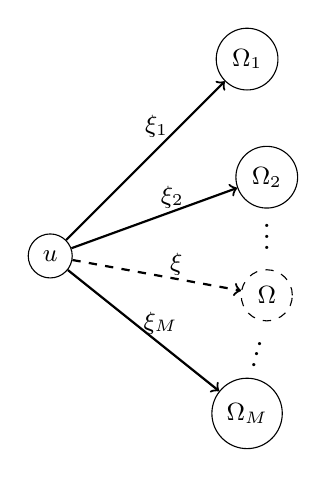
\begin{tikzpicture}

\draw (.5,.5) node(ROOT)[circle,draw]{\small $u$ };
\draw (3,3) node(ONE)[circle,draw]{ \small $\Omega_1$ };
\draw (3.25,1.5) node(TWO)[circle,draw]{ \small $\Omega_2$ };
\draw (3.25,.85) node(DOTONE){ \large $\vdots$ };
\draw (3.25,0) node(N)[circle,dashed,draw]{ \small $\Omega$ };
\draw (3.15,-.65) node(DOTTWO)[rotate=-15]{ \large $\vdots$ };
\draw (3,-1.5) node(S)[circle,draw]{ \small $\Omega_M$ };

\draw (1.85,2.15) node(OMG1){ \small $\xi_1$ };
\draw (2.05,1.25) node(OMG2){ \small $\xi_2$ };
\draw (2.1,.4) node(OMG){ \small $\xi$ };
\draw (1.9,-.35) node(OMGS){ \small $\xi_M$ };

\draw[thick, ->] (ROOT) -- (ONE) ;
\draw[thick,->] (ROOT) -- (TWO);
\draw[thick,dashed, ->] (ROOT) -- (N);
\draw[thick,->] (ROOT) -- (S);

%\draw[thick,dashed] (TWO) -- (N);
%\draw[thick,dashed] (N) -- (S);

\end{tikzpicture} 
\caption{Scenario Tree for Two Stage Problem}
  \label{fig:mip}
\end{figure}

The objective is to allocate a budget for capacity additions in order to reduce the expected blackout size.  $W_{in}$ is the cost of load shed at bus $i$ in node $n$ of the scenario tree.  Let $u$ be the vector of capacity additon and $w$ be a vector of binary variables representing whether that transmission element gets new capacity.  $B_u$ and $B_w$ is the budget for capacity expansion.
\begin{subequations}

\begin{align} \displaystyle
	{\large \mbox{min}} \hspace{10px} &  \Expect_\Xi \sum_{in} \left[c^2_{in}  x^2_{in,m} + c^1_{in} x_{in,m}   + W_{in} (\hat{d}_{i} - d_{in,m}) \right]	\\
	&(d,x,y,z)_m  \in \Omega(\xi_m)    \hspace{20px}   \forall \xi_m \in \Xi	\\
	& \underline{X}_e w_e \le u_e \le \overline{X}_e w_e \hspace{35px} \forall e \in \cE\\
	&\sum_e u_e \le B_u 	\\
	& \sum_e w_e \le B_w  
\end{align}
\label{TX}
\end{subequations}
\subsection{Computational Implementation}
The model outlined in (\ref{TX}) is solved using Gurobi 4.5.  The stopping criteria was either a 40\% optimality gap or 10,000s.  The program was run for several different expansion budgets, with both the total budget and the maximum number of lines being changed.  The output of this model is a vector $u$ which represents the amount of capacity to add to each power line on the grid.  This is used to modify the initial grid and run the OPA simulation to find the effects it has on the system.  In order to find out whether these solutions are reasonable or not, a heuristic was developed to compare against.

The heuristic used is based on a large number of OPA simulation runs in which the power lines were ranked in descending order based on the percentage of runs in which that given power line has failed.  Then, for a given total budget $B_u$ and maximum number of changed lines $B_w$, the heuristic picks the top $B_w$ lines in the list and then distributes the budget $B_u$ evenly over the lines.  The OPA simulation is used to compare the results of the two models.  Since the MSIP was calibrated based on the 4 contingencies, a second set of 4 random initial contingencies to start the OPA process to evaluate the effects.




\begin{figure}
 \centering
	\begin{tikzpicture}
		\begin{axis}[xlabel=$LS$ (MW), ylabel=$P($Load Shed $> LS )$
				,legend pos=north east
				,grid=major,
				,xmin=-25,xmax=1300
				,title=\mbox{Load Shed Distribution} ]


 	\addplot[red,line width=2pt] table[x=ls, y=prob] {./data/d25k20.dat};
	\addlegendentry{design}
	
	\addplot[blue,line width=2pt] table[x=ls, y=prob,mark=square] {./data/dumb25k20.dat};
	\addlegendentry{heuristic}

	\addplot[black,line width=2pt] table[x=ls, y=prob,mark=square] {./data/sim.dat};
	\addlegendentry{nom}




		\end{axis}	
	\end{tikzpicture}
  \caption{Load Shed Distribution for the OPA simulation and MSIP formulation}
 \label{dist}
\end{figure}

In \Cref{dist}, we see that we were able to shift the load shed distribution using the design $u$ found from the MSIP solution of \Cref{TX}.  In order to evaluate the solution, we ran the OPA simulation and compared against a simple heuristic.  The heuristic used the results of a number of trials of the OPA simulation and distributed capacity evenly among the 10 lines which had failed the most.  This strategy did reasonably well.  The MSIP was able to beat this strategy on some occasions, but not always.  The MSIP has a coarse representation of the underlying uncertainty due to the computational difficulty in solving a multi-stage stochastic program.  The size of the scenario tree was 4 stages with 3 outcomes per node, and even when it was this small, there was often at least a 40\% optimality gap.

% Calibrate ---------------------------------------------------------

\section{Conclusion}
%After several trials, we found this solution methodology to be inadequate.  Due to the computational difficulty, the stochastic tree could only have around 4 stages with 3 outcomes per node in ideal settings by trial and error.  When using 4 initial contingencies, only sometimes were solutions found within a 40\% optimality gap.  This coarse representation of the underlying uncertainty made it a poor representation of the effects of the decision variables on the OPA simulation.  However, this approach may be successful if more analysis could determine highly probable failure sequences which need to be protected against.

Using the OPA simulation as a reference for how the grid may respond to cascading power failures, a mixed integer model was developed which represents the cascading effects over a fixed number of outcomes and stages.  While this model can be difficult computationally due to the decision dependent uncertainty, it is extremely flexible.  The model can be used to include cascading effects in a wide range of power system problems with optimality criteria ranging from least cost to minimize worst-case problems.  A computation example was done on transmission expansion, which showed the model was able to better than a reasonable heuristic, even though it was only solved to a 40\% optimality gap.  Future work can be done in order to improve the solve time for these types of models based on techniques developed in stochastic and mixed integer optimization.

%\theendnotes
%\setcounter{endnote}{0}

